
\chapter{Конструкторская часть}\label{Konstruct}
%\addcontentsline{toc}{chapter}{2 Конструкторская часть}

\section{Схемы алгоритмов}\label{SchemaAlg}


\subsection{Схема стандартного алгоритма умножения матриц}\label{SchemaMatrixMultiply}

На рисунке \ref{ris:schemabubble} показана схема алгоритма сортировки пузырьком.

\begin{figure}[H]
  \center{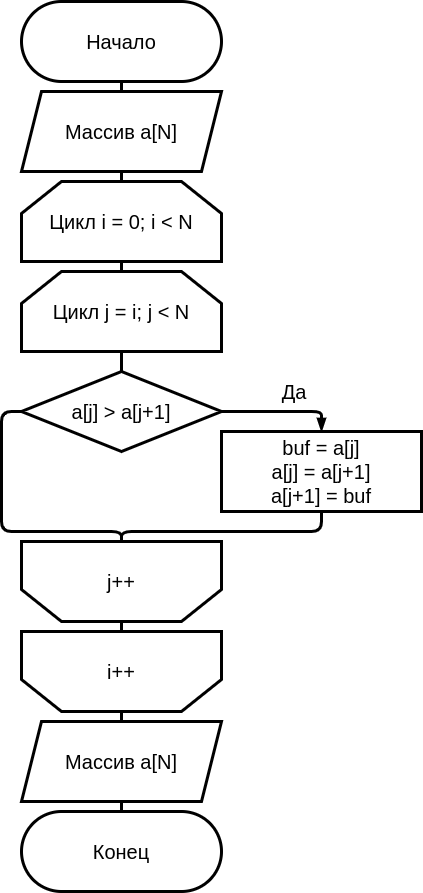
\includegraphics[scale=0.35]{l1.bubble}}
  \caption{Схема алгоритма сортировки пузырьком}
  \label{ris:schemabubble}
\end{figure}

На рисунке \ref{ris:schemachoise} показана схема алгоритма сортировки выбором.

\begin{figure}[H]
  \center{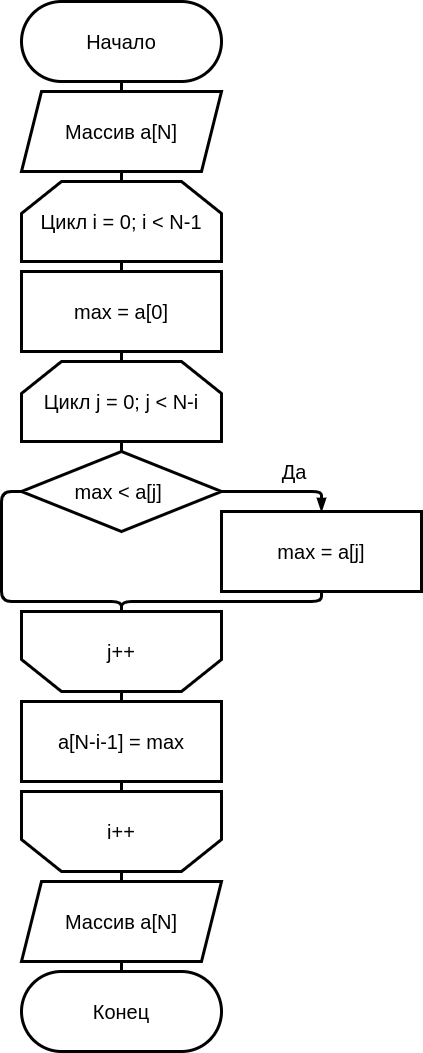
\includegraphics[scale=0.35]{l1.choise}}
  \caption{Схема алгоритма сортировки выбором}
  \label{ris:schemachoise}
\end{figure}

На рисунке \ref{ris:schemainsert} показана схема алгоритма сортировки вставками.

\begin{figure}[H]
  \center{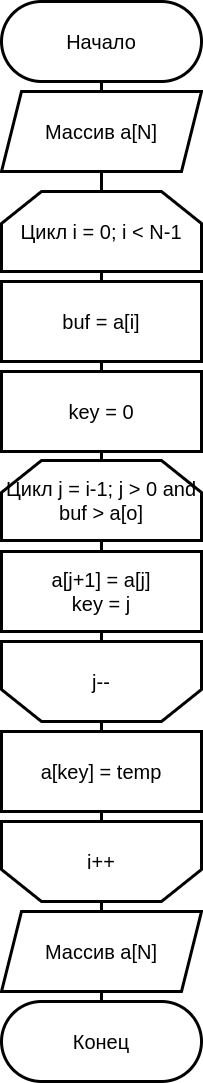
\includegraphics[scale=0.35]{l1.insert}}
  \caption{Схема алгоритма сортировки вставками}
  \label{ris:schemainsert}
\end{figure}


\section{Трудоемкость алгоритмов}\label{Complecity}

\subsection{Трудоемкость алгоритма сортировки пузырьком}\label{ComplecityBubble}

Трудоемкость в лучшем случае $ O(n^2) $:

$ f = 2 + N \cdot (2 + 2 + N \cdot (2 + 3)) = 5\cdot N^2 + 4 \cdot N + 2$\label{formula:complecitybubblegood}

Трудоемкость в худшем случае $ O(n^2) $:

$ f = 2 + N \cdot (2 + 2 + N \cdot (2 + 3 + 9)) = 14\cdot N^2 + 4\cdot N + 2$\label{formula:complecitybubblebad}
 

\subsection{Трудоемкость алгоритма сортировки выбором}\label{ComplecityChoise}

Трудоемкость в лучшем случае $ O(n^2) $:

$ f = 2 + N \cdot (2 + 2 + 4 + 2 + N \cdot (2 + 2)) = 4\cdot N^2 + 10 \cdot N + 2$\label{formula:complecitychoisegood}

Трудоемкость в худшем случае $ O(n^2) $:

$ f = 2 + N \cdot (2 + 2 + 4 + 2 + N \cdot (2 + 2 + 2) = 6\cdot N^2 + 10 \cdot N + 2$\label{formula:complecitychoisebad}

\subsection{Трудоемкость алгоритма сортировки вставками}\label{ComplecityInsert}

Трудоемкость в лучшем случае $ O(n) $:

$ f = 2 + N \cdot (2 + 3 + 2) = 7 \cdot N + 2$\label{formula:complecityinsertgood}

Трудоемкость в худшем случае $ O(n^2) $:

$ f = 2 + N \cdot (2 + 3 + 2 + 2 + N \cdot (2 + 5) = 7\cdot N^2 + 9 \cdot N + 2$\label{formula:complecityinsertbad}

\section{Сравнительный анализ трудоемкостей алгоритмов}\label{Konstructanalis}

Сравнив трудоемкости, можно сделать вывод, что в лучшем случае самым быстрым алгоритмом из рассматриваемых является алгоритм сортировки
вставками, самый медленный - сортировка пузырьком. В худшем случае самый быстрый алгоритм - сортировка выбором, самый медленный - 
сортировка пузырьком.

\section{Структуры данных}\label{Structs}

При реализации приведенных алгоритмов потребуется тип данных: массив.

\section{Тестирование}\label{Testing}

\subsection{Классы эквивалентности}\label{TestingClasses}

Для алгоритма умножения матриц можно выделить следующие классы эквивалентности:

\begin{enumerate}
    \item отсортированный по возрастанию массив
    \item отсортированный по убыванию массив 
    \item случайный массив
\end{enumerate}

\subsection{Способы тестирования}\label{TestingMethods}

При разработке программы удобно использовать следующие методы тестирования:

\begin{enumerate}
    \item Модульные тесты 
    \item Функциональные тесты 
\end{enumerate} 

\section{Вывод конструкторской части}\label{KonstructResult}
На основе данных, полученных в аналитическом разделе, были построены схемы используемых алгоритмов,
выделены необходимые для реализации структуры данных и методы тестирования.

